\subsection{Microaneurysm (MA) detection}

\begin{frame}\frametitle{Motivation I}

\par MAs are early symptoms of diabetic retinopathy

\begin{table}[]
\centering
\begin{tabular}{|p{3cm}|p{8cm}|}
\hline
Disease severity lvl & Findings observable upon dilated ophthalmoscopy \\ \hline
None & No abnormalities \\ \hline
Mild NPDR & \bf{Microaneurysms (MA) only} \\ \hline
Moderate NPDR & More than just MA but less than severe NPDR \\ \hline
\multirow{4}{*}{Severe NPDR} & \multirow{4}{*}{\begin{tabular}[c]{@{}l@{}}
$>$20 intraretinal hemorrhages in each quad \\
{\bf{or}} Definite venous beading in 2+ quads \\
{\bf{or}} Intraretinal microvascular anomalies in 1+ quad \end{tabular}} \\
 &  \\
 &  \\
 &  \\ \hline
PDR & \begin{tabular}[c]{@{}l@{}}Neovascularization\\ {\bf{or/and}} Vitreous/preretinal hemorrhage\end{tabular} \\ \hline
\end{tabular}
\end{table}

\par \href{http://www.icoph.org/downloads/Diabetic-Retinopathy-Detail.pdf}{International Clinical Diabetic Retinopathy Disease Severity Scale, Detailed Table: http://www.icoph.org/downloads/Diabetic-Retinopathy-Detail.pdf}

\end{frame}

\begin{frame}\frametitle{Motivation II}
\par We have problems with detection of early symptoms
\par
\begin{figure}
\begin{center}
\vspace{-10pt}
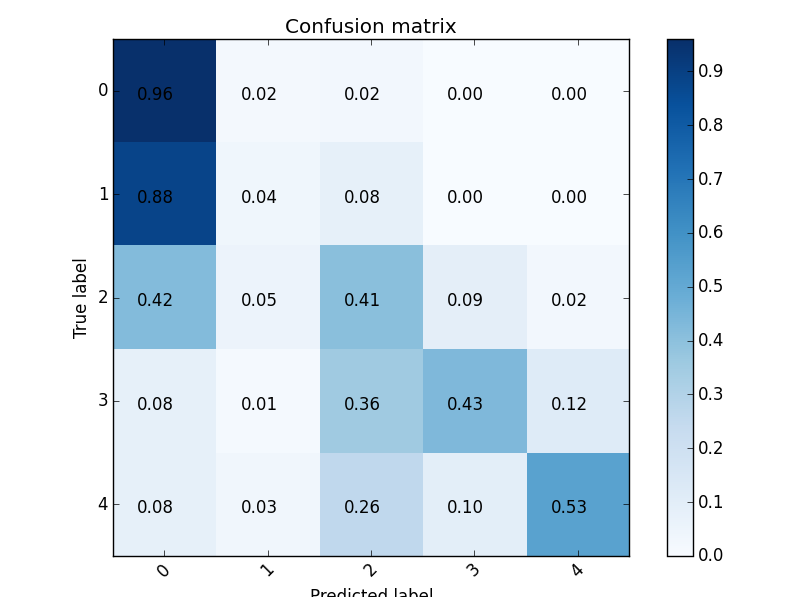
\includegraphics[width=0.4\textwidth]{pics/submission_21_inner_squares_conv5_maxout.png}
\caption{Confusion matrix on 128x128 pixels input}
\vspace{-15pt}
\end{center}
\end{figure}

\par MA have round shape with $2-5$ pixels in radius on $1024\times1024$ image 
\par MA became invisible after downsampling to 128x128/256x256
\par $\Rightarrow$ Classes 0,1,2 almost indistinguishable due to low resolution
\vspace{0.5cm}
\par We have not enough resources\&data to learn on highres images
\par $\Rightarrow$ Let's try plain old image processing

\end{frame}

\begin{frame}\frametitle{Bag of visual words}
\par Detector: Hessian blob detector
\par Feature extractors: HOG, LBP
\par Examples of found blobs: negatives and positives
\par per-class plots of features after PCA
\par conclusion: not worked :-(
\end{frame}

\begin{frame}\frametitle{Microaneurysm candidates using the determinant of the Hessian}
\par SHORT INTRO TO HESSIAN BLOB DETECTION

\par By considering the scale-normalized determinant of the Hessian, also referred to as the 
\[ \operatorname{det} HL(x, y; t) = t^2 (L_{xx} L_{yy} - L_{xy}^2) \]
where $HL$ denotes the Hessian matrix of $L$ and then detecting scale-space maxima of this operator one obtains another straightforward differential blob detector with automatic scale selection which also responds to saddles

\[(\hat{x}, \hat{y}; \hat{t}) = \operatorname{argmaxlocal}_{(x, y; t)}(\operatorname{det} H L(x, y; t))\]
\end{frame}

\begin{frame}\frametitle{Microaneurysm candidates}
\centering
\only<1>{
\begin{tabular}{|@{}c@{}|@{}c@{}|@{}c@{}|@{}c@{}|@{}c@{}|}
\hline

Normal & Mild & Moderate & Severe & Proliferative \\

\hline
	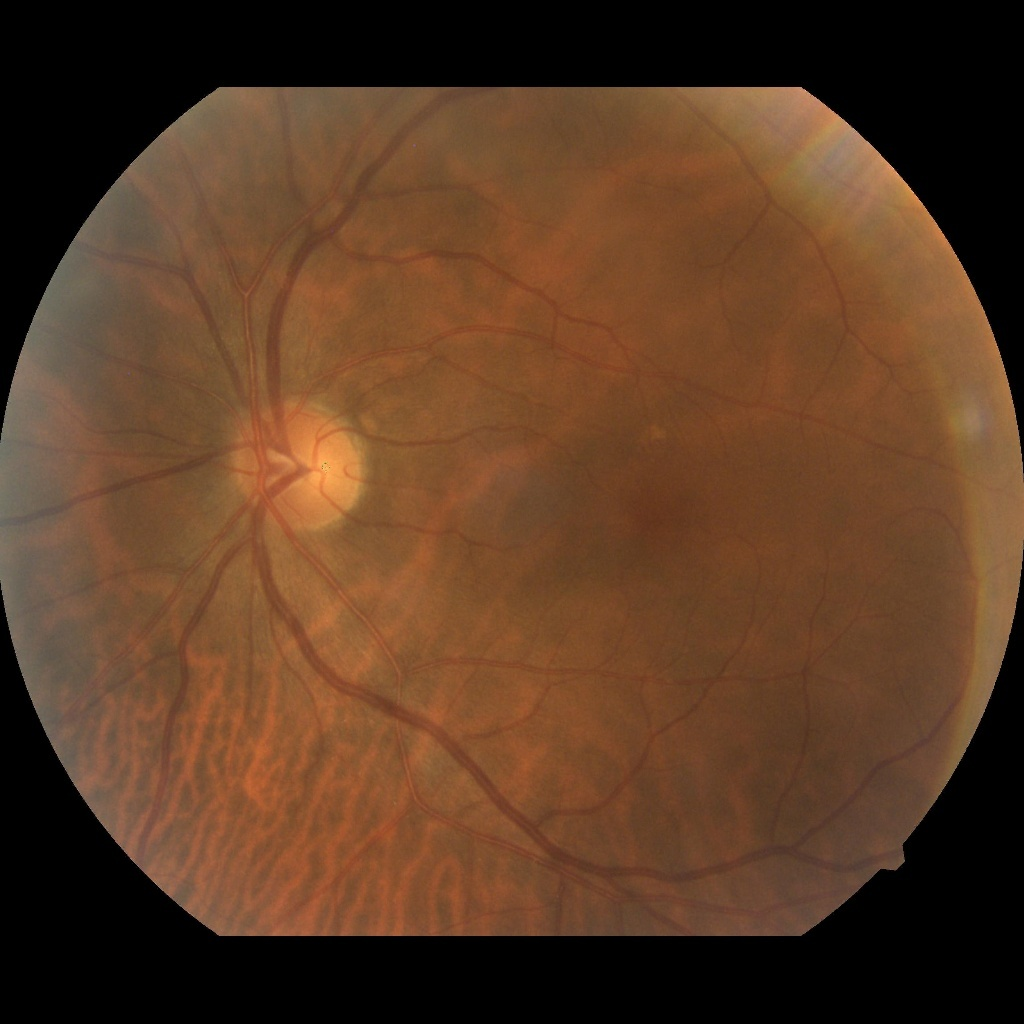
\includegraphics[width=0.2\textwidth]{pics/classified_samples/197_left_0.jpg} &
	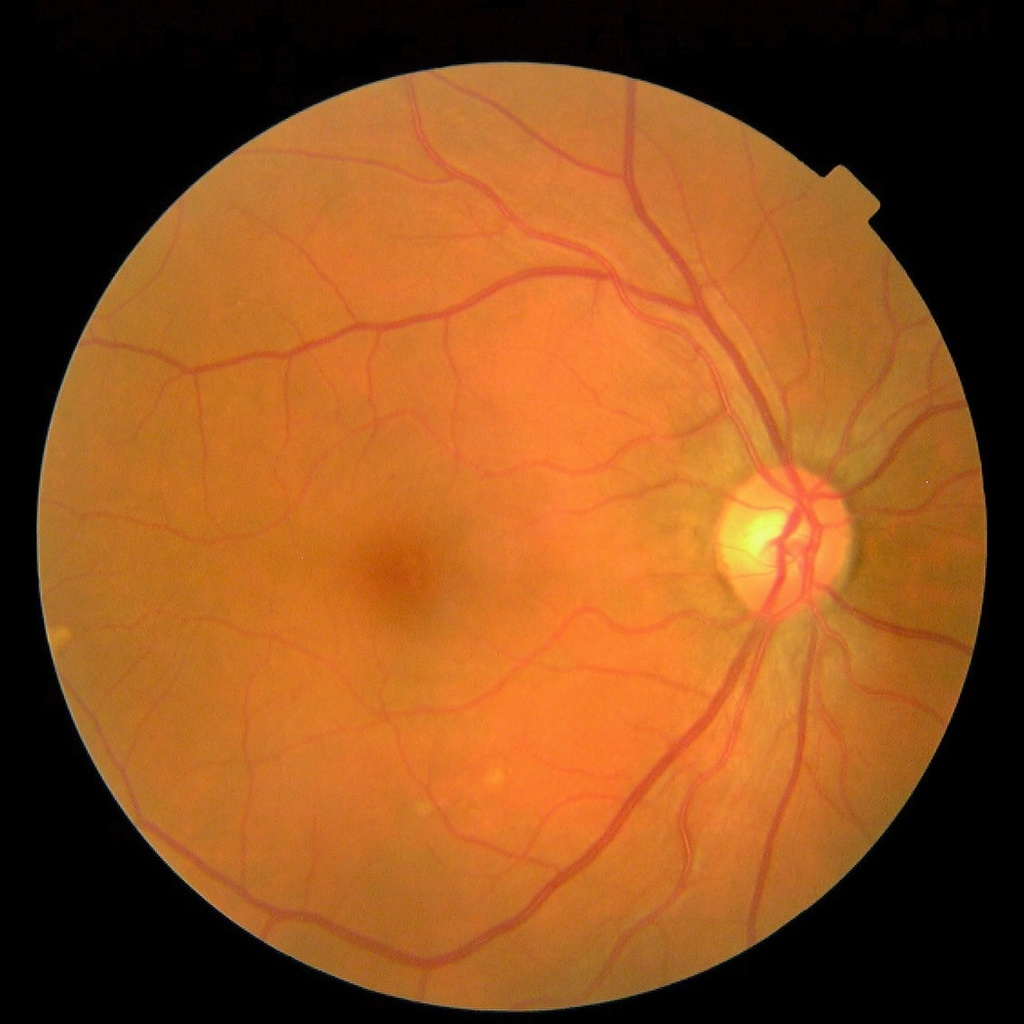
\includegraphics[width=0.2\textwidth]{pics/classified_samples/204_right_1.jpg} &
	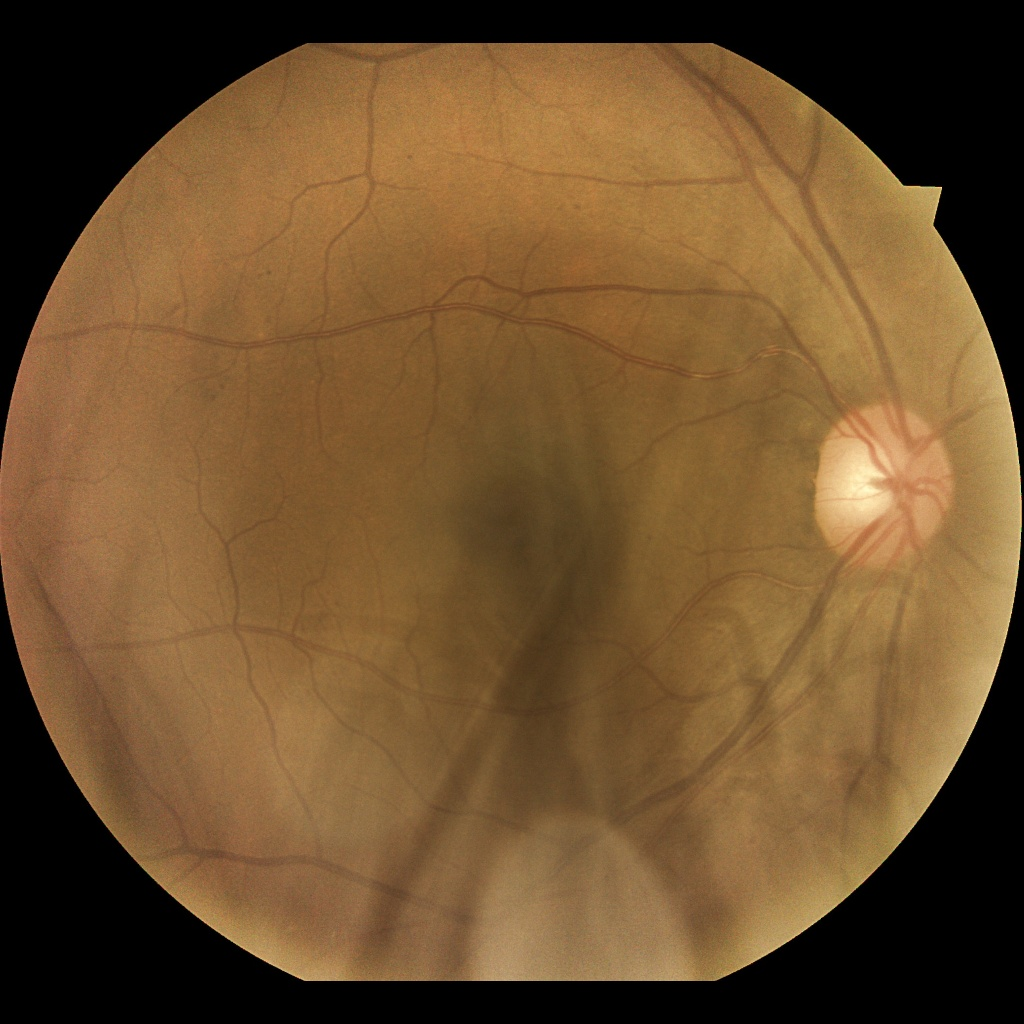
\includegraphics[width=0.2\textwidth]{pics/classified_samples/82_right_2.jpg} &
	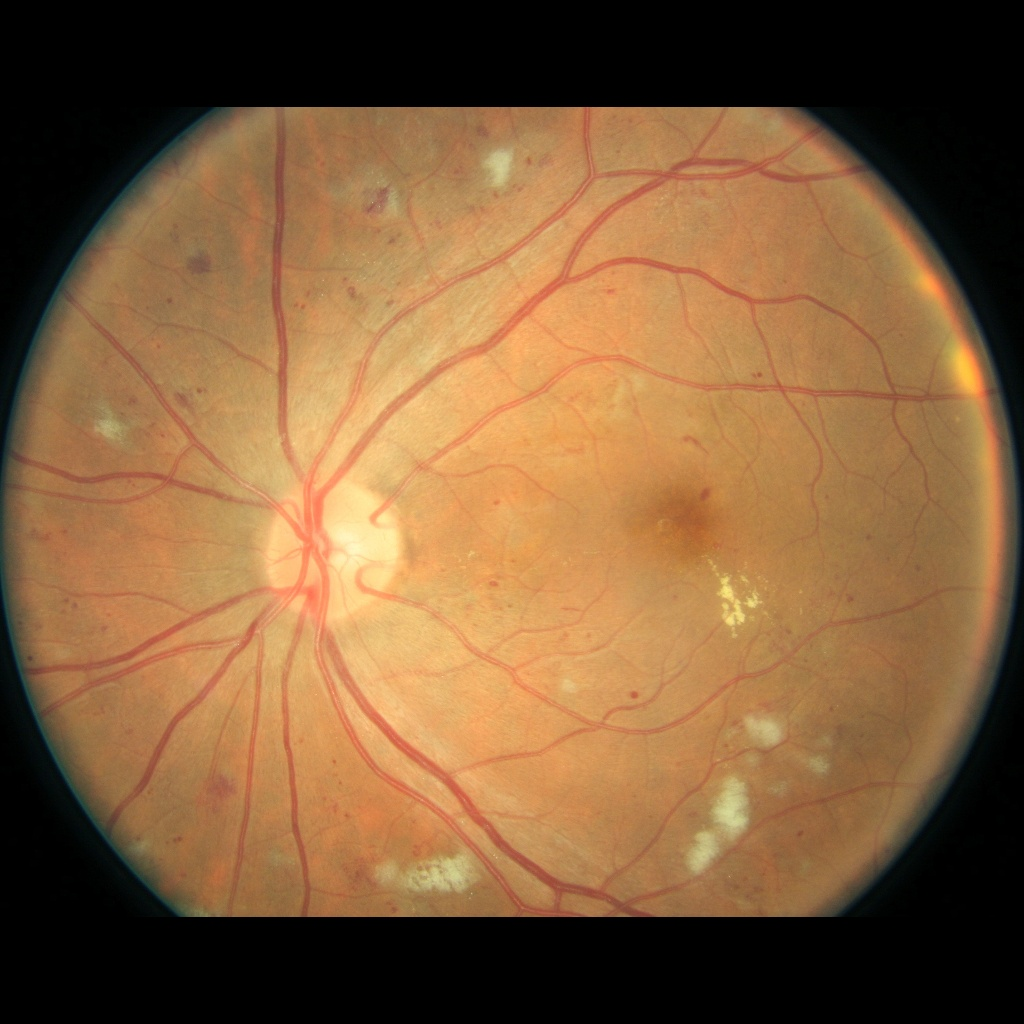
\includegraphics[width=0.2\textwidth]{pics/classified_samples/687_right_3.jpg} &
	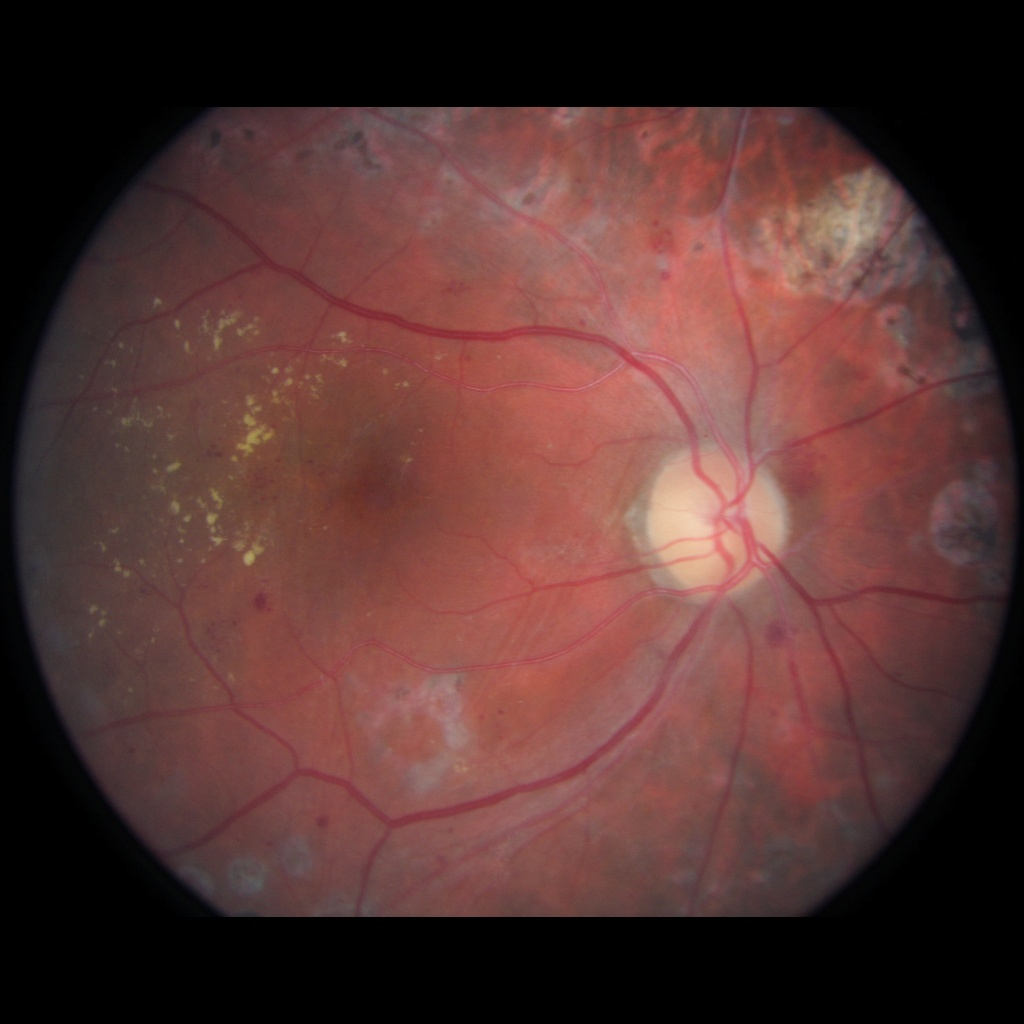
\includegraphics[width=0.2\textwidth]{pics/classified_samples/2496_left_4.jpg} \\\noalign{\vspace{-0.15cm}}
\hline
	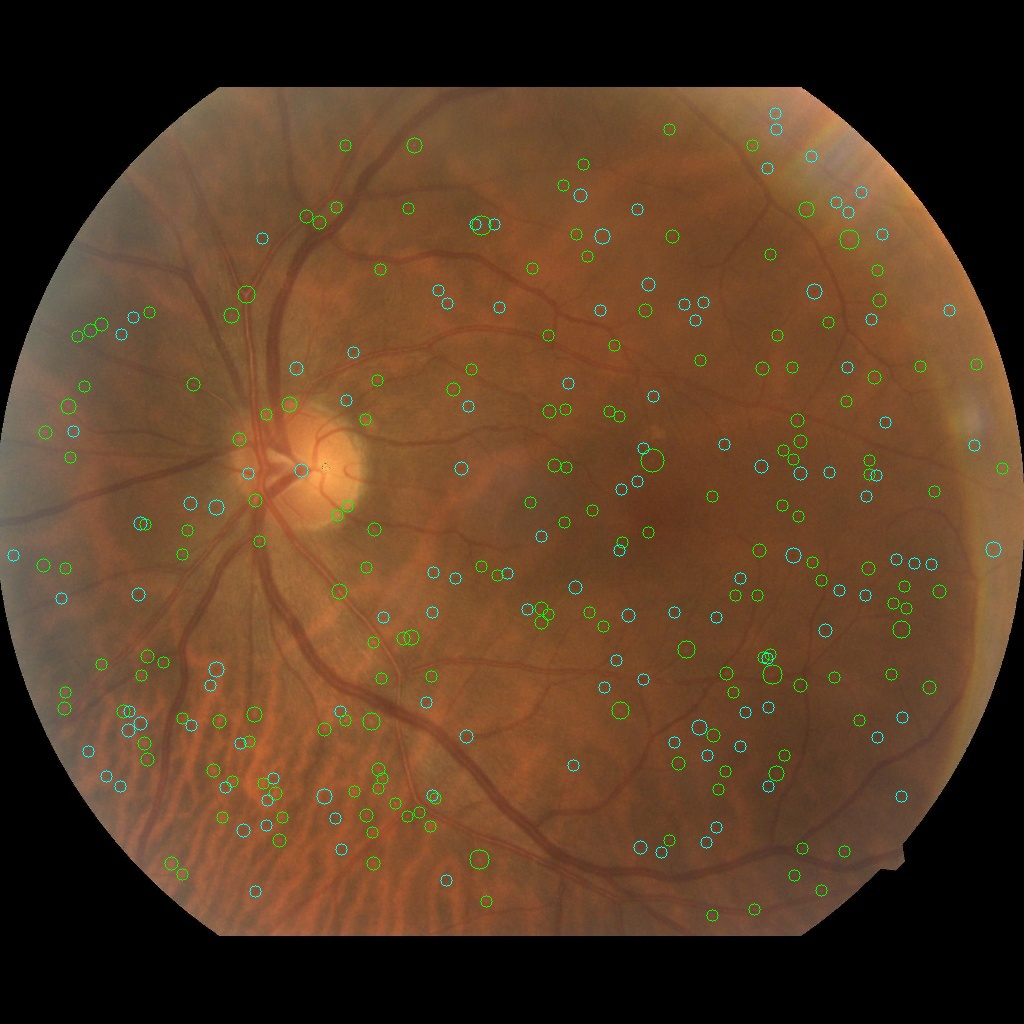
\includegraphics[width=0.2\textwidth]{pics/classified_samples/197_left_0_blobs.jpg} &
	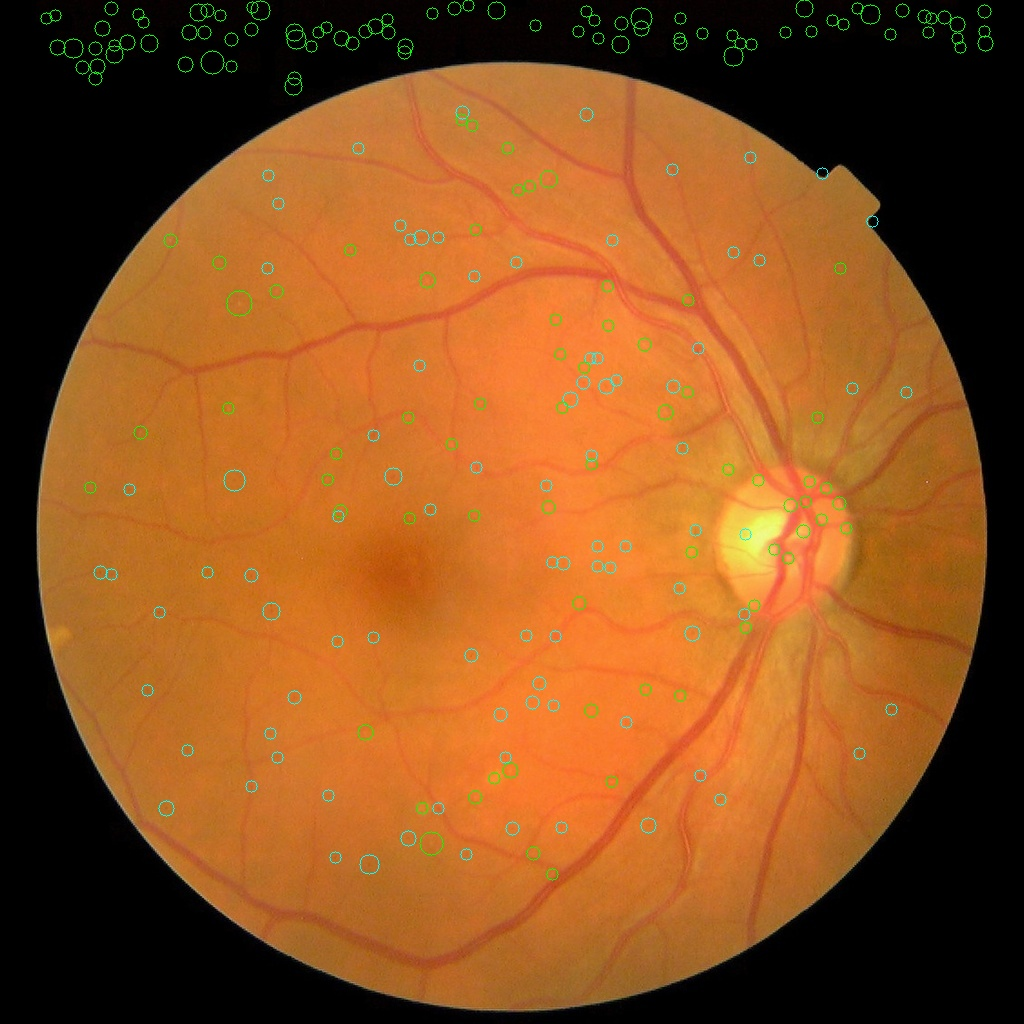
\includegraphics[width=0.2\textwidth]{pics/classified_samples/204_right_1_blobs.jpg} &
	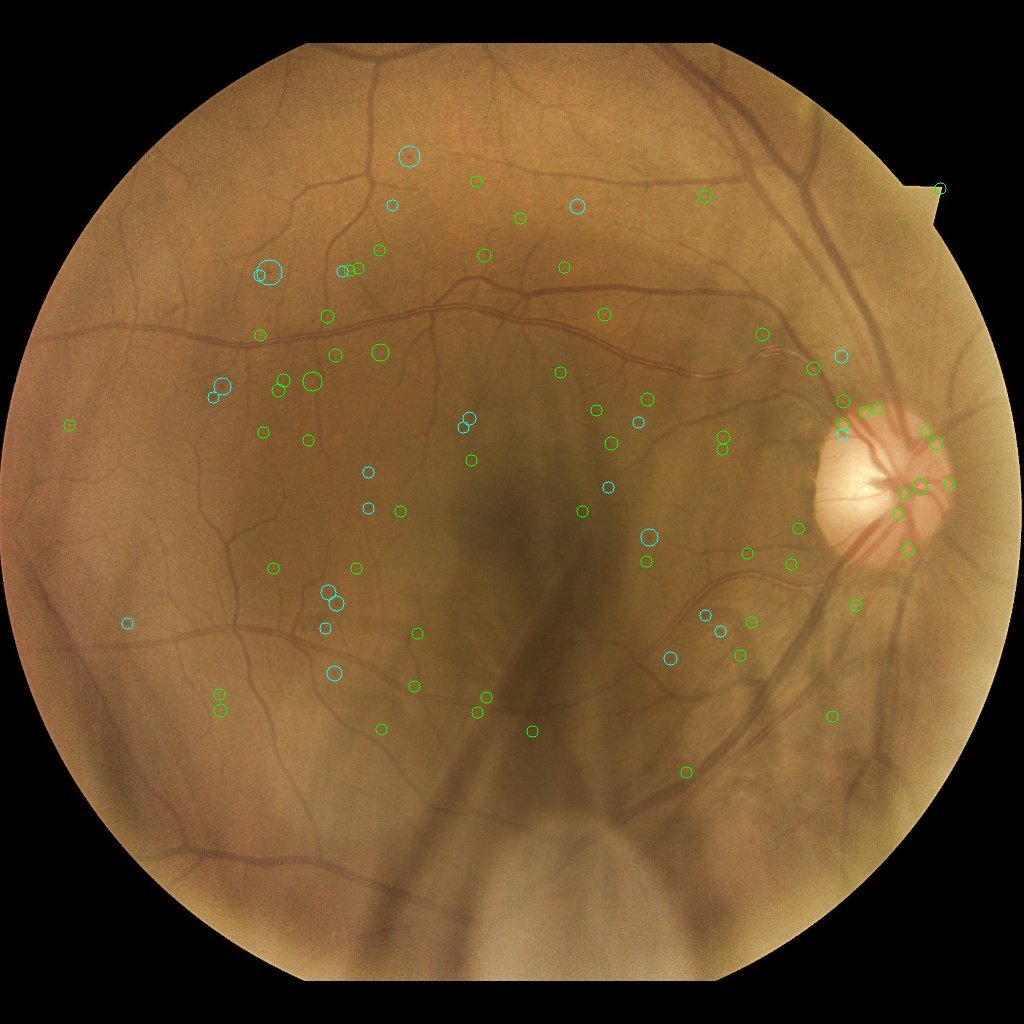
\includegraphics[width=0.2\textwidth]{pics/classified_samples/82_right_2_blobs.jpg} &
	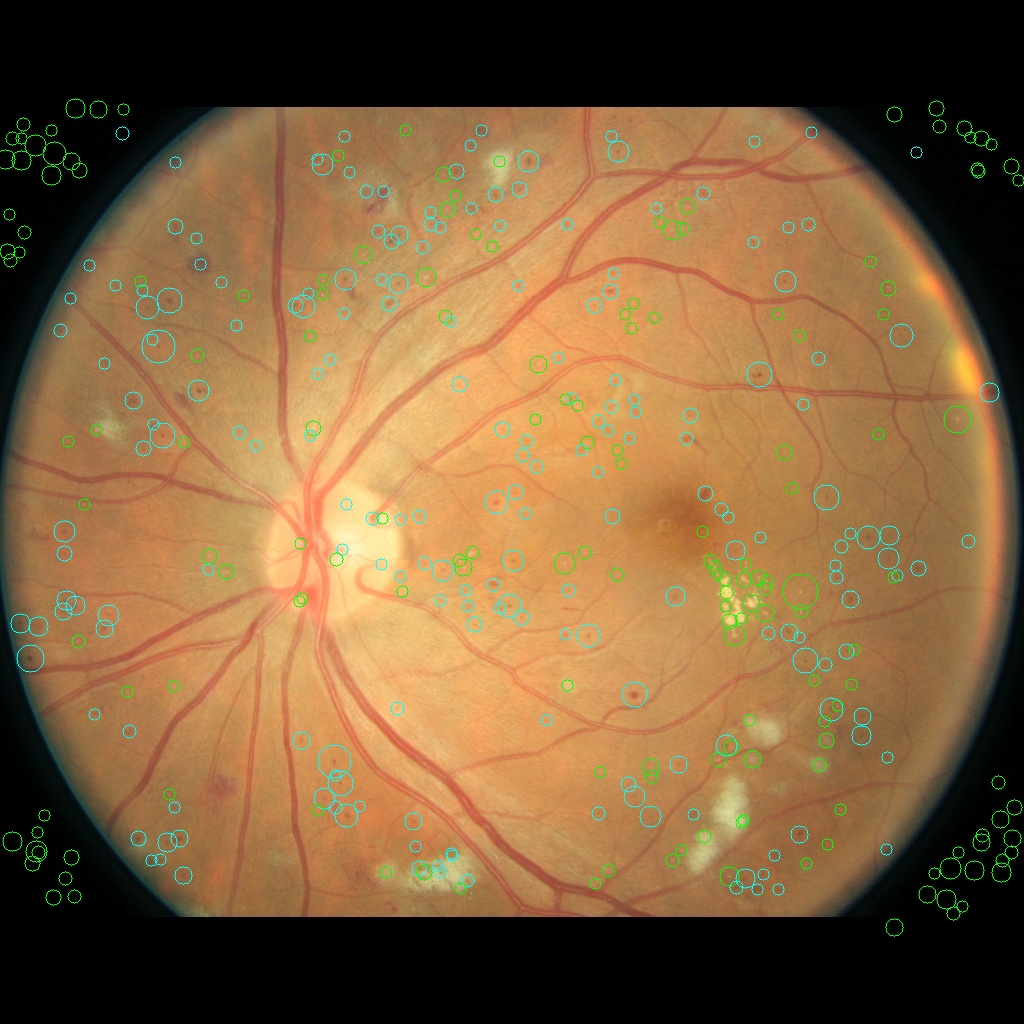
\includegraphics[width=0.2\textwidth]{pics/classified_samples/687_right_3_blobs.jpg} &
	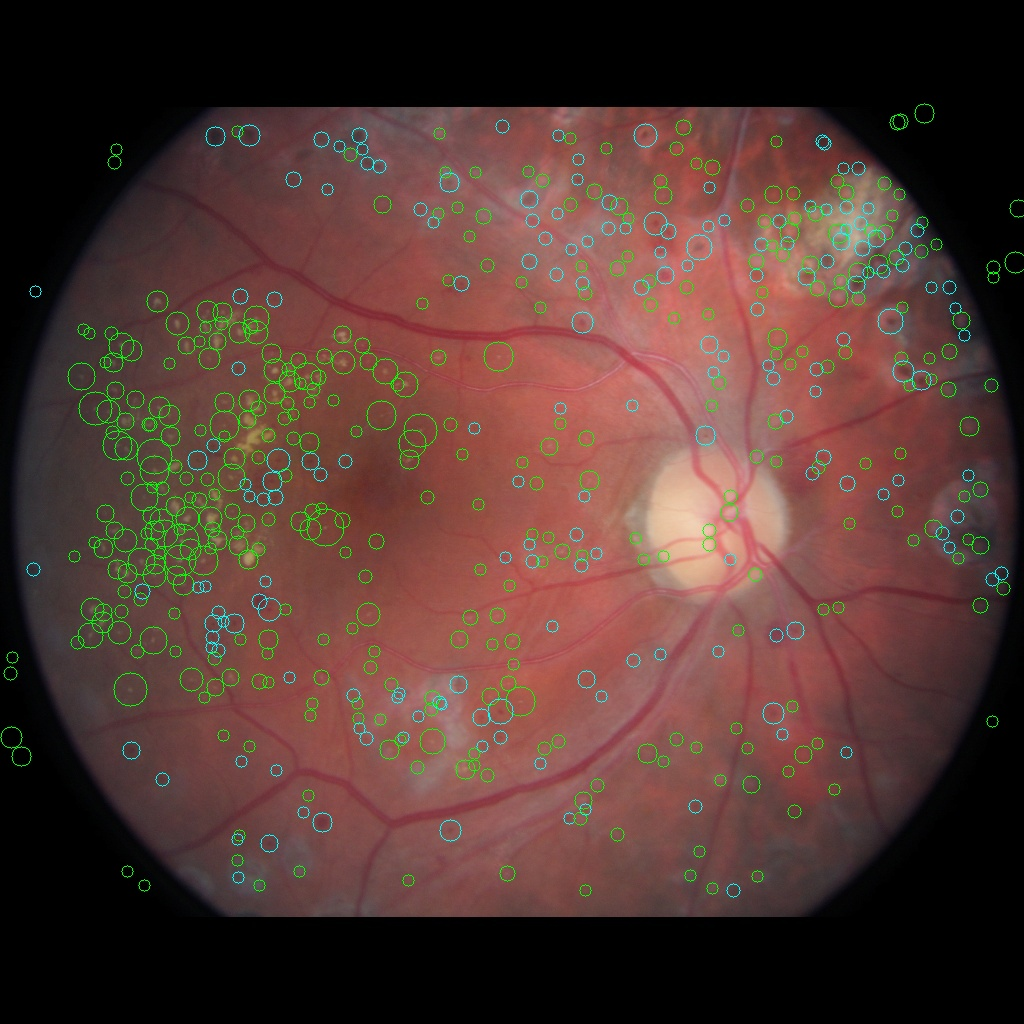
\includegraphics[width=0.2\textwidth]{pics/classified_samples/2496_left_4_blobs.jpg} \\

\end{tabular}
}

\only<2>{
	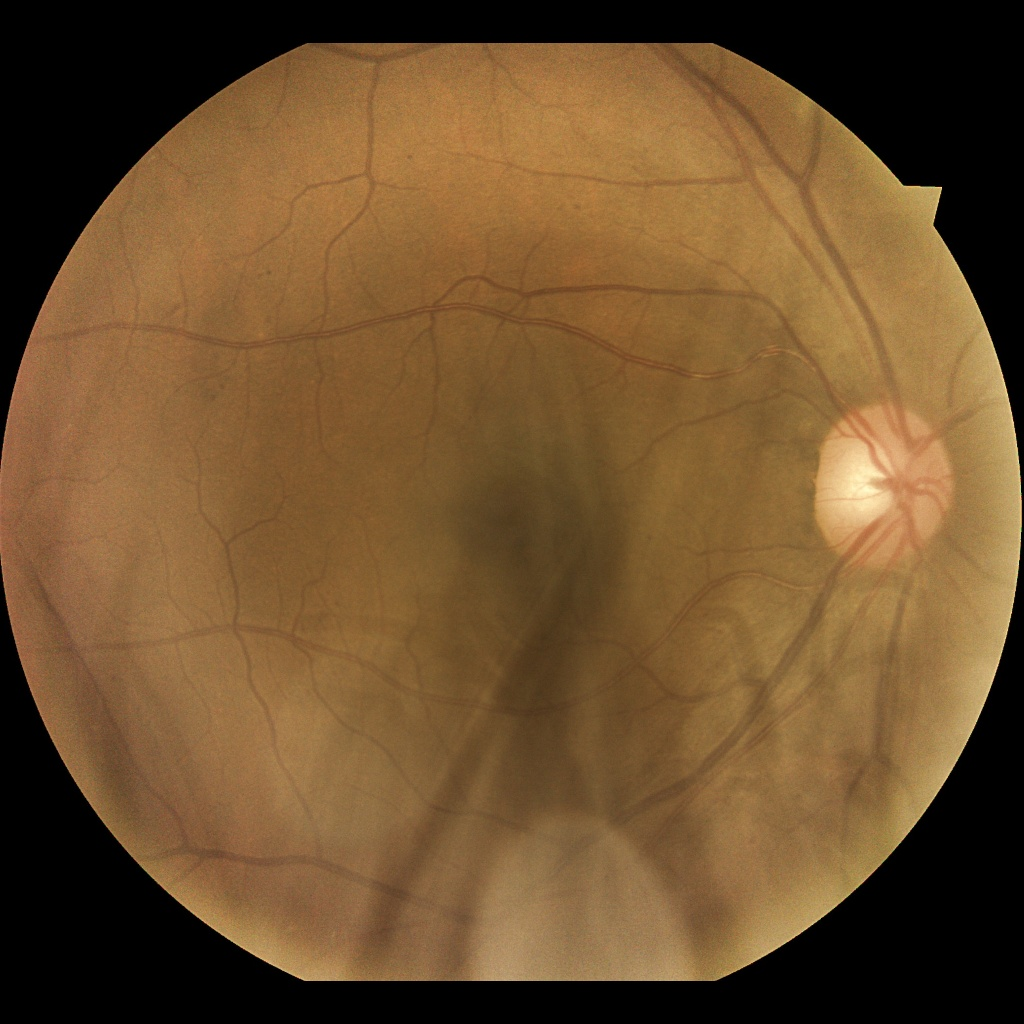
\includegraphics[width=0.65\textwidth]{pics/classified_samples/82_right_2.jpg}
}

\only<3>{
	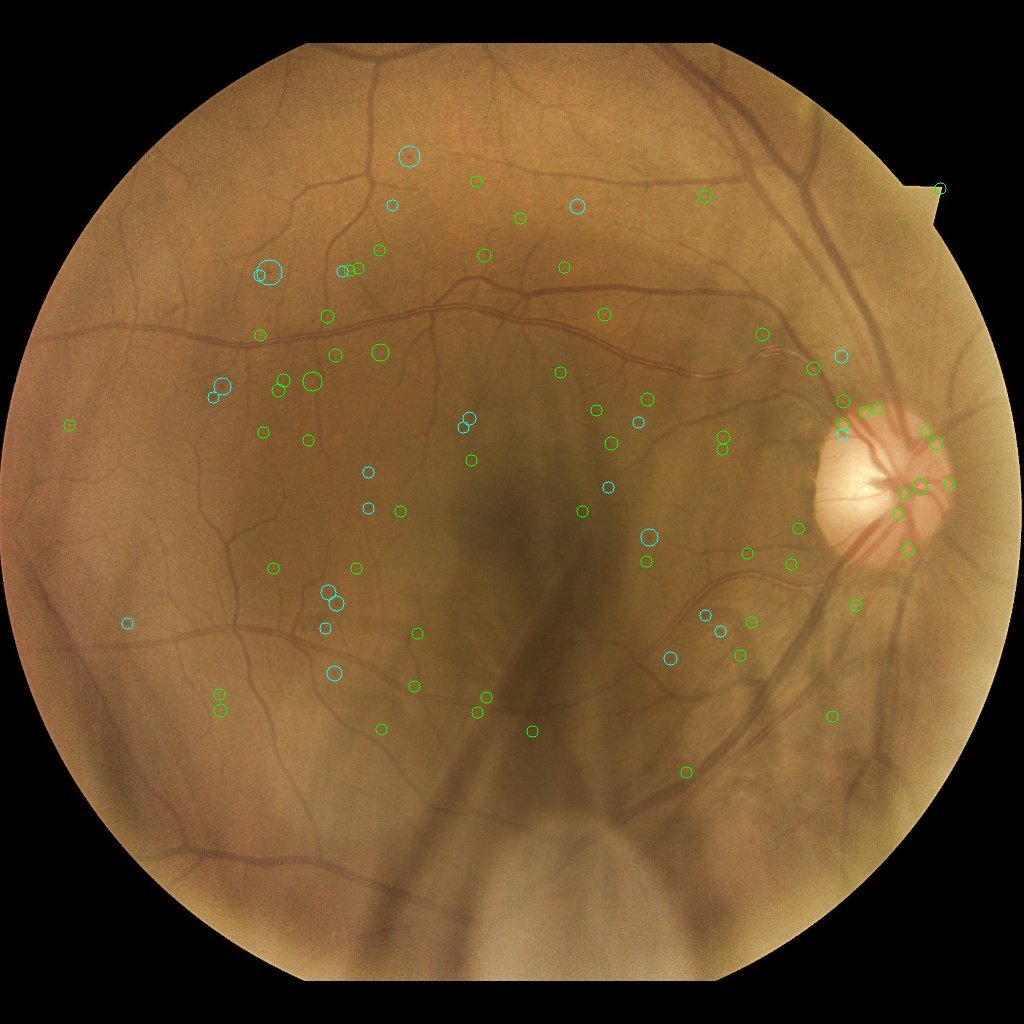
\includegraphics[width=0.65\textwidth]{pics/classified_samples/82_right_2_blobs.jpg}
}
	
\end{frame}

\begin{frame}\frametitle{How blobs looks}

\begin{center}
\begin{tabular}{| b{0.15\linewidth} |@{}c@{}|@{}c@{}|@{}c@{}|@{}c@{}|@{}c@{}|}
\hline
strength & $\sigma = 1.7$ & $\sigma = 3.4$ & $\sigma =  5.1$ & $\sigma = 6.8$ & $\sigma = 8.0$ \\

\hline
$[300,450)$ & 
	\includepatches{patches_300_450_1_2_raw.pdf} & 
	\includepatches{patches_300_450_3_4_raw.pdf} & 
	\includepatches{patches_300_450_5_6_raw.pdf} & 
	\includepatches{patches_300_450_6_7_raw.pdf} & 
	\includepatches{patches_300_450_7_9_raw.pdf} \\

\hline
$[450, 600)$ & 
	\includepatches{patches_450_600_1_2_raw.pdf} & 
	\includepatches{patches_450_600_3_4_raw.pdf} & 
	\includepatches{patches_450_600_5_6_raw.pdf} & 
	\includepatches{patches_450_600_6_7_raw.pdf} & 
	\includepatches{patches_450_600_7_9_raw.pdf} \\
	
\hline
$[600, 750)$ & 
	\includepatches{patches_600_750_1_2_raw.pdf} & 
	\includepatches{patches_600_750_3_4_raw.pdf} & 
	\includepatches{patches_600_750_5_6_raw.pdf} & 
	\includepatches{patches_600_750_6_7_raw.pdf} & 
	\includepatches{patches_600_750_7_9_raw.pdf} \\

\hline
$[750, \infty)$ & 
	\includepatches{patches_750_5000_1_2_raw.pdf} & 
	\includepatches{patches_750_5000_3_4_raw.pdf} & 
	\includepatches{patches_750_5000_5_6_raw.pdf} & 
	\includepatches{patches_750_5000_6_7_raw.pdf} & 
	\\

\hline
\end{tabular}
\end{center}
\end{frame}


\begin{frame}\frametitle{How blobs looks}

\begin{center}
\begin{tabular}{| b{0.15\linewidth} |@{}c@{}|@{}c@{}|@{}c@{}|@{}c@{}|@{}c@{}|}
\hline
strength & $\sigma = 1.7$ & $\sigma = 3.4$ & $\sigma =  5.1$ & $\sigma = 6.8$ & $\sigma = 8.0$ \\

\hline
$[300,450)$ & 
	\includepatches{patches_300_450_1_2_scaled.pdf} & 
	\includepatches{patches_300_450_3_4_scaled.pdf} & 
	\includepatches{patches_300_450_5_6_scaled.pdf} & 
	\includepatches{patches_300_450_6_7_scaled.pdf} & 
	\includepatches{patches_300_450_7_9_scaled.pdf} \\

\hline
$[450, 600)$ & 
	\includepatches{patches_450_600_1_2_scaled.pdf} & 
	\includepatches{patches_450_600_3_4_scaled.pdf} & 
	\includepatches{patches_450_600_5_6_scaled.pdf} & 
	\includepatches{patches_450_600_6_7_scaled.pdf} & 
	\includepatches{patches_450_600_7_9_scaled.pdf} \\
	
\hline
$[600, 750)$ & 
	\includepatches{patches_600_750_1_2_scaled.pdf} & 
	\includepatches{patches_600_750_3_4_scaled.pdf} & 
	\includepatches{patches_600_750_5_6_scaled.pdf} & 
	\includepatches{patches_600_750_6_7_scaled.pdf} & 
	\includepatches{patches_600_750_7_9_scaled.pdf} \\

\hline
$[750, \infty)$ & 
	\includepatches{patches_750_5000_1_2_scaled.pdf} & 
	\includepatches{patches_750_5000_3_4_scaled.pdf} & 
	\includepatches{patches_750_5000_5_6_scaled.pdf} & 
	\includepatches{patches_750_5000_6_7_scaled.pdf} & 
	\\

\hline
\end{tabular}
\end{center}
\end{frame}